% Leonhard Schatt

\section{Versuchsaufbau zur Bestimmung der spektralen Empfindlichkeit}



Der Versuchsaufbau wird wie in Abbildung \ref{Versuch1} gezeigt aufgebaut. Dabei wird das Licht einer 150 W Xe-Bogenlampe auf einen Monochromator gestrahlt. 
Dieser, ein Gittermonochromator mit Gitterkonstante $1180 \mathrm{mm}^{-1}$, führt das Licht weiter auf einen Strahlteiler, welcher 50\% des Lichtes 
durchlässt und 50\% auf das Power-Meter lenkt. Der durchgelassene Strahl wird von einem Chopper moduliert, bevor das Licht auf die Solarzelle 
fällt. Der Lock-in Verstärker erhält sein Referenzsignal vom Chopper. Die Solarzelle ist kurzgeschlossen. Dabei wird der Kurzschlussstrom ermittelt, indem 
man jenen auf einen U/I-Wandler leitet und die von diesem ausgegebene Spannung auf den Lock-in Verstärker gibt. 

\begin{figure}[ht]
    \captionsetup{justification=centering,margin=2cm}
    \centering
    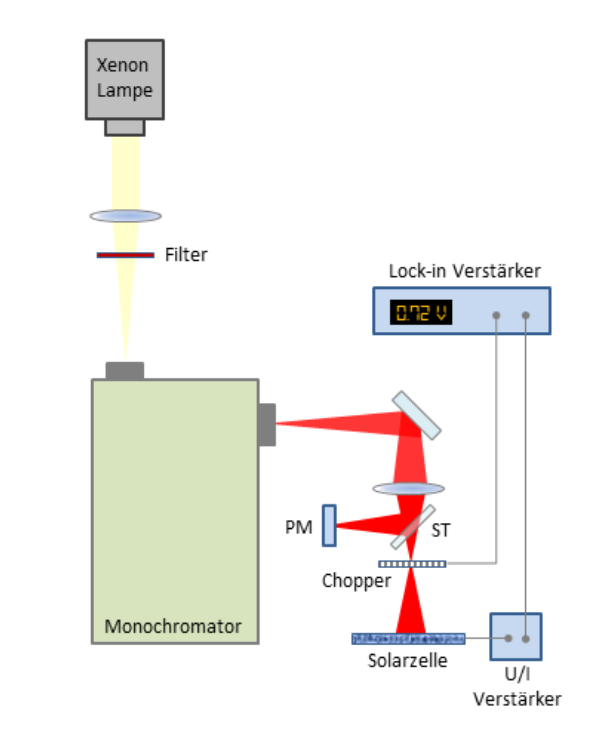
\includegraphics[width =7cm]{Bilder/Versuchsaufbau1.png}
    \caption{Versuchsaufbau zur Bestimmung der spektralen
    Empfindlichkeit. PM: Power-Meter, ST: polka-dot Strahlteiler
    }
    \label{Versuch1}
\end{figure}

Die Wellenlänge des Lichtes, welches auf der Solarzelle ankommt, wird durch ein Drehrad an der Seite des Monochromators eingestellt. Dabei muss ab 
Wellenlänge größer als 600nm wurde ein Kantenfilter vorgeschoben, um die Beugungsmaxima höherer Ordnung abzublocken. Gemessen werden in 
beiden Versuchsteilen jeweils die Module mono-Si, multi-Si und CIS. Dabei wird 
Licht im Bereich 300-1200nm betrachtet. Die Dateien mit den Rohdaten befinden sich im Anhang.


\section{Messung der Strom-Spannungs-Kennlinie}

Bei dieser Messung wird der Aufbau wie in Abbildung \ref{Versuch2} verwendet. Der Baustrahler ist in diesem Fall die Lichtquelle. Dieser steht hinter zwei 
Glasscheiben, welche die Infrarotstrahlung abhalten sollen, damit sich die Solarzelle nicht so stark erhitzt. Außerdem wird die Solarzelle mit 
einem Ventilator gekühlt. Der Abstand, welcher mit einem Stelltransformator betrieben wird, steht in einem Abstand von circa 50cm zur Solarzelle. 
 
\begin{figure}[ht]
    \captionsetup{justification=centering,margin=2cm}
    \centering
    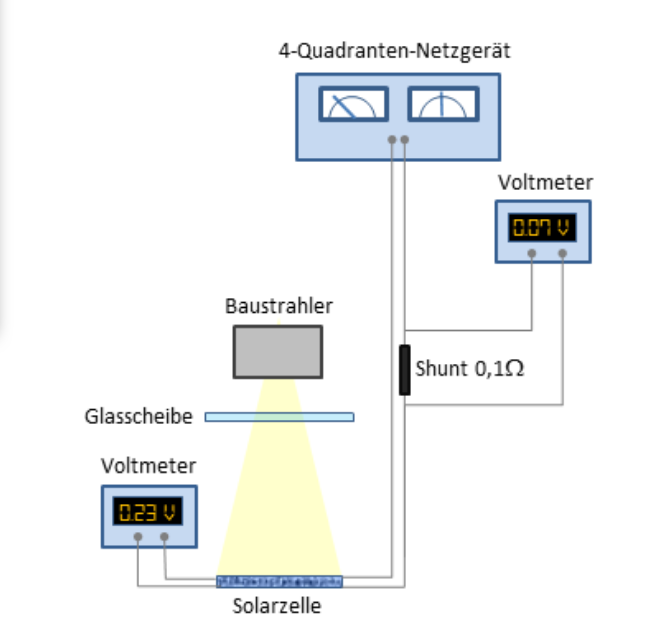
\includegraphics[width =8cm]{Bilder/Versuchsaufbau2.png}
    \caption{ersuchsaufbau zur Messung der Strom-Spannungs-Kennlinie}
    \label{Versuch2}
\end{figure}

Der Spannungsabfall wird dabei über einen hochpräzisen 0.1$\Omega$ Shunt gemessen. 
Gemessen werden Intensitäten bis 0.25sun. Dies wird bewerkstelligt, indem man am Stelltransformator die Werte 130V, 180V und 230V einstellt.
Außerdem verwendet man ein Vier-Quadraten--Netzgerät um die U-I-Kennlinien zu messen. Solange der Anstieg in der Kurve mit der Spannungsregelung noch kontrollierbar ist,
 verwendet am besten Diesen. Um das Modul vor zu hohen Strömen zu schützen, schaltet man danach auf den Stromregelungsmodus.
Gemessen wir in einem Wertebereich von -1V bis 1A, beziehungsweise bei dem CIS Modulnur bis 40mA.
Vor jeder Messung wird die Beleuchtungsstärke mit einer kalibierten Solarzelle gemessen. Bei den größeren Modulen werden 5 Messwerte genommen 
und anschließend gemittelt, um das ungleichmäßige Strahlen des Baustrahlers zu berücksichtigen. Die Messwerte werden an den Ecken und in der Mitte genommen. 
Die kalibrierte Solarzelle hat dabei die Kalibration 282mA/sun. Diese wird wieder über einen hochpräzisen Shunt von 0.1 $\Omega$ gemessen. 

